% Schematic pathwise reflection at the FIRST hit of the horizontal barrier a.
% Coordinates after tau are exact mirror images in y=a. Not simulated Brownian data.
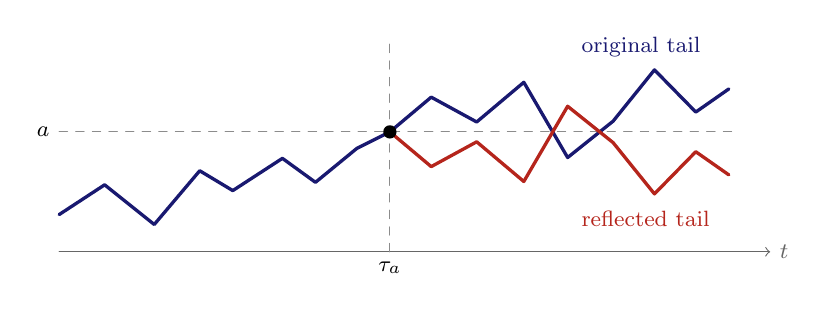
\begin{tikzpicture}[x=1.05cm,y=1.05cm,line cap=round,line join=round]
 \draw[->,black!60] (0,-0.45)--(8.6,-0.45) node[right,font=\footnotesize] {$t$};
 \draw[black!45,dashed] (0,1)--(8.2,1);
 \node[anchor=east,font=\footnotesize] at (0,1) {$a$};
 \draw[black!45,dashed] (4,-0.45)--(4,2.15);
 \node[anchor=north,font=\footnotesize] at (4,-0.45) {$\tau_a$};
 \draw[MidnightBlue,very thick]
   (0,0)--(0.55,0.36)--(1.15,-0.12)--(1.7,0.53)--(2.1,0.29)--(2.7,0.68)--(3.1,0.39)--(3.6,0.8)--(4,1)
   --(4.5,1.42)--(5.05,1.12)--(5.62,1.6)--(6.15,0.69)--(6.7,1.13)--(7.2,1.75)--(7.7,1.24)--(8.1,1.52);
 \draw[BrickRed,very thick]
   (4,1)--(4.5,0.58)--(5.05,0.88)--(5.62,0.4)--(6.15,1.31)--(6.7,0.87)--(7.2,0.25)--(7.7,0.76)--(8.1,0.48);
 \fill[black] (4,1) circle (2.4pt);
 \node[anchor=west,text=MidnightBlue,font=\footnotesize] at (6.2,2.03) {original tail};
 \node[anchor=west,text=BrickRed,font=\footnotesize] at (6.2,-0.05) {reflected tail};
\end{tikzpicture}
